\chapter{Weryfikacja pracy robota}
\label{ch:07}

\section{Sposób testowania}

Testy platformy mobilnej można podzielić na dwa etapy. Pierwszy z nich polegał na weryfikacji ilości impulsów zliczonych przez enkodery podczas ruchu robota. Był to kluczowy etap, pozwalający na wczesne wykrycie ewentualnych niedokładności związanych z algorytmem sterującym. 

Drugi etap można nazwać właściwym procesem jakości algorytmów sterowania, ponieważ odbywał się on w warunkach zbliżonych do rzeczywistych. Robot poruszał się zgodnie z preprogramowaną ścieżką, natomiast weryfikacja była możliwa dzięki naklejonej taśmie malarskiej zgodnie z wytyczoną drogą. Był to prosty i efektywny sposób testowania jakości algorytmów. 


\section{Wykryte i usunięte błędy}


\subsection{Błąd nieskończonej pracy silników}
Ważnym aspektem wykrytym w pierwszej fazie testów było niepoprawne zatrzymanie silników. Jeżeli silniki nie pracowały jednakowo, to znaczy, ich odczyty impulsów enkoderów nie były do siebie zbliżone, istniało duże ryzyko nieskończonej pracy silników. 

Powodem takiego niepożądanego działania był warunek zakończenia pracy silników - fragment kodu znajduje się w spisie [\ref{fig:pseudokod:pid}]. Widoczna instrukcja warunkowa sprawdza czy wartość bezwzględna błędu ruchu jest mniejsza niż wartość stałej tolerancji niedokładności. Jeżeli wartość błędu jest wyższa, naturalnie silniki pracują zgodnie z mocą wyznaczoną przez regulator PID, jeżeli natomiast wartość jest niższa, silniki zostają zatrzymane. Ze względu na pewną bezwładność elementów wykonawczych, mimo ich zatrzymania w pewnej iteracji \textit{n}, w kolejnej iteracji \textit{n+1} wartość błędu będzie wynosić więcej niż stała tolerancji. Z tego powodu silniki ponownie rozpoczną pracę nieskończenie zwiększając wartość błędu. 

W związku z powyższym, została dodana flaga widoczna w spisie [\ref{fig:pseudokod:pid}], zapewniająca poprawność działania kodu w każdych warunkach. Jeżeli silnik raz osiągną wartość założoną, flaga uniemożliwia ponowne wejście programu do wznowienia pracy silnika. Stan zmiennej binarnej zostaje zmieniony dopiero po otrzymaniu nowych instrukcji z komputera nadrzędnego. 

\subsection{Błąd odbierania i wysyłania poleceń}
Podczas testów przeprowadzonych w fazie pierwszej, zaobserwowane zostało problematyczne zachowanie komunikacji między SBC Raspberry Pi a kontrolerem silników Ardunino UNO R3. Błąd polegał na zbyt wczesnym wysyłaniu kolejnych poleceń. Z pozoru łatwy do rozwiązania problem, okazał się nie tak trywialny. 

Pierwsza wersja komunikacji polegała na stałym opóźnieniu z wykorzystaniem metody dostarczanej przez klasę \english{time} - \textit{sleep()}. Metoda ta umożliwia uśpienie wątku na określony czas (w sekundach). To podejście ma bardzo poważną wadę - jest nieelastyczne względem wysyłanych komunikatów. Oznacza to, że niezależnie od odległości jaką robot ma przebyć, kolejna komenda zostanie wysłana na przykład po czterech sekundach. 

Kolejnym podejściem, było zastosowanie pewnej flagi lub znacznika, który umożliwi określenie zakończenia pracy robota oraz wykorzystanie go jako warunku kontynuowania. W tym celu dotychczas istniejący kod został umieszczony wewnątrz pętli \textit{while}, co umożliwiło poprawne oczekiwanie na ukończenie zadania. 

Po zastosowaniu wyżej opisanego podejścia, opóźnienie było tak małe, że w warunkach rzeczywistych nieosiągalne, co zmusiło autora do dodania pewnego dodatkowego krótkiego opóźnienia między kolejnymi komendami. 

\subsection{Błąd dokładności jazdy}

Poważnym problemem okazała się dokładność jazdy platformy mobilnej. Mimo, że względem wczesnych wersji algorytmów zostały poczynione znaczne postępy, robot nie osiągnął idealnej dokładności, w szczególności podczas obrotów. 

Pierwsze wersje sterowania opierały się na obrocie względem układu współrzędnych, którego środek znajdował się w punkcie styku jednego koła z podłożem. Innymi słowy, robot obracał się o zadany kąt poruszając się tylko jednym kołem, co nie do końca spełniało wymaganie projektowe, jakim było zastosowanie napędu różnicowego. Dokładność osiągnięta w tej konfiguracji była jednak zadowalająca. 

Po wprowadzeniu napędu różnicowego, pojawiły się większe błędy wynikające z mniej dokładnego zliczania impulsów o znaku ujemnym, a więc podczas ruchu kół do tyłu. Wymagania projektowe zostały spełnione, jednak kosztem dokładności, która we wczesnych wersjach była nienajlepsza. 

\hspace{1cm}

Ostatecznie została podjęta decyzja o zlikwidowaniu jednego kanału enkodera. Ze względu na charakter sterowania robotem, rozróżnienie kierunku jazdy może zostać zrealizowane programowo, zgodnie z tym, co zostało zaprezentowane w kodzie [\ref{fig:enc-count}]. Decyzja ta była spowodowana sposobem zliczania impulsów - za pomocą przerwań globalnych. Przy dużej ilości generowanych przerwań, szybkość mikrokontrolera mogła być niewystarczająca. Dzięki zredukowaniu zliczanych impulsów o połowę, wpływ późnienia wynikającego z dużej ilości generowanych przerwań również został zmniejszony. 

Szczególnie mocno różnica zarysowuje się w przypadku obrotów. Wynika to z faktu, że wcześniej z nieznanych do końca przyczyn, silniki obracały się o nieco mniejszy kąt do tyłu niż do przodu. Efekt pozostawał bez zmian nawet po próbach bezpośredniej ingerencji w postaci dodania stałej ilości impulsów w przypadku obrotu do tyłu lub zwiększenia wartości sygnału PWM. Zachowanie to może wynikać między innymi z jakości wykonania silnika. 

Po zastosowaniu jednego kanału enkodera, opisane problemy zostały zmniejszone, a dokładność znacznie się poprawiła. Nie jest ona jednak idealna. Autor uważa, że największe różnice wprowadziłaby zmiana elementów wykonawczych - silników. Zastosowane silniki firmy Pololu stanowią solidną bazę do rozwoju budżetowych projektów, jednak w przypadku, gdy robot ma realnie funkcjonować niezawodnie w pewnym niekrótkim horyzoncie czasu, należy zastosować zdecydowanie bardziej dokładne silniki z mniejszymi luzami. 

\hspace{1cm}

Dodatkowo ze względu na nieidealną dokładność, autor wprowadził koncepcję stacji dokujących [\ref{fig:stacja}] znajdujących się bezpośrednio przed podajnikiem oraz miejscami docelowymi. Umożliwiają one korekcję toru jazdy, tym samym niwelując błędy powstałe podczas pracy robota. Podobne podejście zostało wymienione w znanej pracy naukowców z Uniwersytetu w Michigan pod tytułem "Where am I", co po polsku znaczy "Gdzie jestem?"\cite{bib:where-am-i}. Wynika z niej, że podczas implementacji algorytmów sterowania opierających się jedynie na odczytach z enkoderów małe błędy, w przypadku powyższego projektu poniżej 1\%, potęgują się w czasie, co uniemożliwia długofalową pracę bez wsparcia na przykład wcześniej wymienionych stacji dokujących.  

\begin{figure}
    \centering
    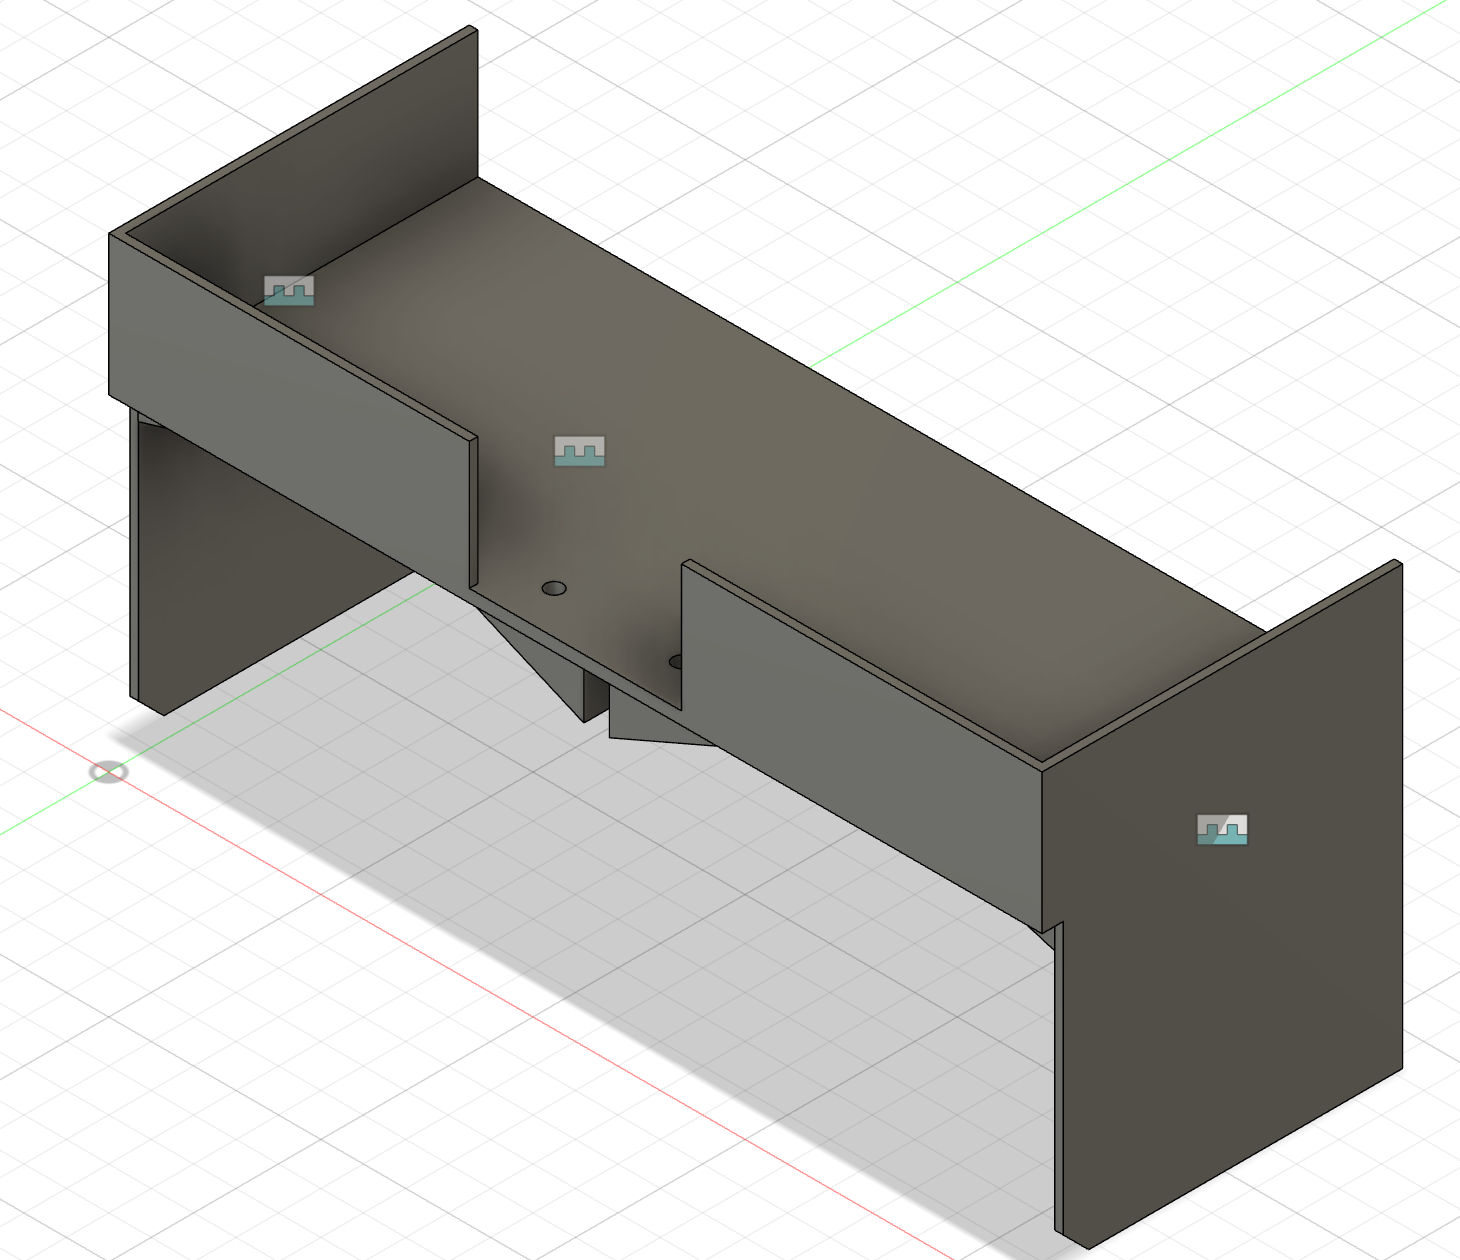
\includegraphics[width=1.0\textwidth]{./graf/upper.png}
    \caption{Zdjęcie przedstawiające stację dokującą oraz miejsce docelowe}
    \label{fig:stacja}
\end{figure}